% Chapter 3

\chapter{Experimental Design}

\label{Chapter4} % 

In this chapter we describe the different methods that were assessed. The methods, in order of gradually increasing sophistication, are as follows:

\begin{enumerate}
    \item Baseline model
	\item Beta-Binomial model
	\item Binary Logistic Regression
	\item Linear SVM Classifier
	\item RBF SVM Classifier
	\item Recurrent Neural Networks
\end{enumerate}

All methods, except for the Bayesian Inference method, require the data to be structured as a time-series. The Bayesian method adopts a different approach that requires the data to be aggregated into half-hourly buckets of a week. The data preparation that was performed is described in the next section, followed by an explanation each method, and the evaluation criteria for assessing the methods in the sections that follow.

\section{Data preparation}

\subsection{Data origination}

The dataset being used in this analysis is the LastFM1k dataset, which is freely available online and contains the listening history of a thousand LastFM listeners. It consists of a series of timestamps denoting when a user started playing a song. We wish to learn the temporal patterns of a user's behaviour in order to predict the next item in the sequence - a play or non-play event. 

The dataset contains the timestamp, user ID, and track ID of users listening habits over a number of years (2005-2009).

\subsection{Data transformation}

The analysis was carried out in Python (via Jupyter notebooks) running on Ubuntu. The raw data consisted of timestamps of when a song was played and a user ID. These were loaded as-is into a SqlLite3 database in order to reduce the need to repeat data preparation steps. The methods themselves utilized Scikit-learn for all models, save for the RNN model which used Tensorflow.

UserIDs were converted to integer (e.g. 'User0005' became '5') and a period lookup table was created at $n$ minute intervals, against which all timestamps in our main dataset were mapped to. $n$ was chosen to be a period of 30 minutes.

The data, which contained entries for the times at which each user listened to music, was supplemented with all the times they did \emph{not} listen to music, between their date of their first and last play.  This was required in order to generate a sequence of play and non-play events. 

\subsection{Feature selection}

The features that were chosen were based on the preliminary analysis (see next chapter) and consisted of time-series and non-time series features. The time-series features were binary, representing play (1) or non-play (0) events at $t, t-1, t-2, t-3, t-4, t-5,  t-12hrs, t-23.5hrs, t-24hrs, t-24.5hrs, t-1wk, t-2wks, t-3wks$, and $t-4wks$.

$t-1$ to $t-5$ represent user activity in the previous 2.5 hours. The remaining time-lags were chosen to represent half-day, daily, and weekly cycles, with additional emphasis around the -24 hour mark due to the daily patterns observed in the preliminary analysis.  

The non-time lag features were binary features representing the day of the week (isMon, isTue etc.) and the number of hours away from 5pm in either direction - so a timestamp at 4pm and 6pm would both be 1. Again this was based on the observations in the preliminary analysis of 5pm being a peak listening hour.

\section{Validation and Test dataset selection}

Our working dataset was a subset of the full 1000 user dataset, and comprised of 4,217,228 rows of training data across 97 users. Of this a random sample of 100,000 rows was taken and 5-fold cross-validation employed.  

\subsubsection{Data Imbalance}

A data imbalance is when the training data is when one or more of the classes is under-represented in the dataset. Of the 4,217,228 rows in our working data set, 361,081 (8.6\%) were play events and 91.4\% were non-play events. This can result in models that achieve a high accuracy score by following either of the following two heuristics:

\begin{itemize}
	\item Predict non-event for everything
	\item Predict $t$ will be the same as $t-1$
\end{itemize}
 
There are several methods for dealing with data imbalance \parencite{Brownlee} including restricting input data, having a weighted loss function, and using recall as an evaluation measure. We used recall as well as weighting. Both class weights and sample weights were employed in the Scikit-learn models. The class weights were inversely proportional to play \& non-play frequencies in the input data, while the sample weights were a hyper-parameter.  In the RNN model only sample weighting was used.

The effect of class weighting is to encourage the model to predict play events. The effect of the sample weighting is to encourage the model to predict play events while minimizing the number of false-positives.

\section{Methods}

\subsection{Baseline Model}

Our baseline model will be to assume that the prediction at time $t$ is the same as the outcome in the prior period, $t-1$. As music listening events tend to be clustered (people listen to music in batches) the accuracy of the baseline model will be fairly high. However it will not be able to predict the first play of a listening session, or where the listening session duration lasts no longer than a single period, which in the experiments is defined as a 30 minute period.

\subsection{Beta-Binomial Model}

The Beta-Binomial model is a simple form of Bayesian Inference. Conceptually it assumes listening habits follow a weekly pattern and can therefore be summarized as the probability of a play event, at any time period within a week.

It therefore divides a week into 336 half-hourly timeslots (30 min timeslots x 336 = 1 week) and builds up a probability table for each timeslot based on the frequency of plays of the entire population. This forms the prior probability of the Beta-Binomial distribution. 
This prior probability is then adapted for each user based on their play history at time $t$. If the user a is a new user, then their history would be empty and as such their probability of listening to music would simply be based on the prior probability derived from the overall population. Fig \ref{fig10b} shows the calculation of the prior for the first 2.5 hours of a Sunday (represented as day-hour-halfhour format). 

\begin{figure}[h!]
	\centering
	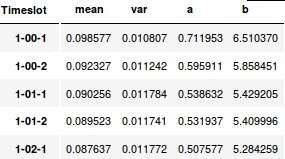
\includegraphics[width=8cm, keepaspectratio,]{fig010b.jpg}
	\caption{}
	\label{fig10b}
\end{figure} 

The mean and var come from the population data, and $a$ and $b$ are derived from these as is usual with a Beta distribution.

If a user does have a play history, given time $t$, then this history can be used in a likelihood function. The likelihood function represents the probability of a user listening to music, and we define this as a binomial distribution, where $k$ is the number of plays they have had in a given period, $n$ is the sum of plays and non-plays, and $\theta$ is the unknown probability parameter for the binomial distribution.

$${n \choose k}\,p^{k}(1-p)^{n-k}$$

As the Beta distribution is a conjugate prior to the Binomial the model can be reduced to: $Beta(\alpha+P, \beta+Q)$ where $P$ is the count of plays and Q is the count of non-plays. For which the parameters $\alpha$ and $\beta$, are derived from the training set, with an estimate of the mean for each half-hourly time period as shown in fig \ref{fig10b}. To do this we first calculate the probability of a play (total plays in period / count of plays and non-plays) per user, then take the mean and variance across users. $a$ and $b$ are then determined as:
$a = (\frac{(1- \mu)}{\sigma} - \frac{1}{\mu}) \mu^2$
and
$\beta=\alpha\left(\frac{1}{\mu}-1\right)$.

Finally we convert the probabilities into a binary outcome by optimizing for a threshold $\lambda$ at which we predict a play event.

An important point to note in all this is how to determine the start and end of a period in which we count up the users listening habits, significantly impacts the model. For example, it would be natural to take the very first song play of a user in our dataset as the date they started listening to music, and start counting the timeslots they listened in from that point forward. But where do we stop counting? The simple approach is to say that the very last record we have of a song play by that user in our dataset represents the end of the counting period. But as fig. \ref{fig23} demonstrates, a users listening profile may not remain constant over time -- they may for instance stop using the music service for many years and then listen again one more time before they stop altogether.

\begin{figure}[h!]
	\centering
	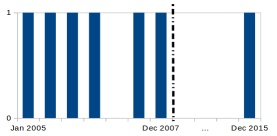
\includegraphics[width=8cm, keepaspectratio,]{fig023.jpg}
	\caption{}
	\label{fig23}
\end{figure} 

The consequence of this is that the probability of listening at a given timeslot in week, decreases substantially if we are counting the large gaps as well. The alternative would be to somehow determine for each user, what counts as a 'typical' listening period and use that to form our prior. This was not considered practical however within this research and therefore the simplistic rule for deriving our prior had to be used. We see in the results chapter that this results in very low probabilities. Despite this, the impact ought to be offset by using a lower probability threshold at which we determine something to be a play event, as we do using a ROC curve in the results chapter.

\subsection{Binary Logistic Regression}

This method (and the subsequent methods) adopts a more classical time-series approach to the prediction problem by constructing a dataset as a sequence of play events at time $T_t = 1$ and non-play events $T_t = 0$, with $t$ representing a time period of a fixed interval of 30 minute chunks.

\begin{figure}[h!]
	\centering
	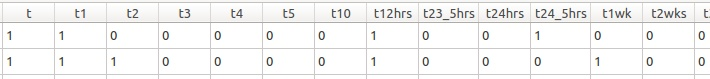
\includegraphics[width=12cm, keepaspectratio,]{fig021.jpg}
	\caption{Example of times-series data}
	\label{fig021}
\end{figure} 

We seek to model the probability of an event in the current time period $t$, given the history of events: $p(Y_t =1 \mid Y_h)$. Our binary logistic model is therefore defined as:
$$p(Y_t = 1|Y_h) = \sigma(w^Tx + b)$$
$$p(Y_t = 1|Y_h) = 1 - p(Y_t = 1|Y_h)$$

with $\sigma$ being the sigmoid function defined as:
$$\sigma(x)=\frac{e^x}{1+e^x}$$

Determining the optimal weights and constant can be determined by maximization of the log-likelihood or the minimization of the negative log-likelihood. 

In addition we will be using an L2 regularizer term,  $ + 1/2w^Tw$, to prevent over-fitting:

\subsection{Linear SVM Classifier}

SVM models work by determining a separation plane between classes based on the support vectors - the data points closes to the decision boundary. A linear SVM regression model performs this through the Epsilon Intensive loss function \parencite{Vapnik}. The objective becomes to \textit{minimize:}

$$max(0,\left\| (y_i - w_i x_i - b) - \epsilon \right\|)$$

In other words we ignore cost functions that are within a certain margin  $\epsilon$. In our case this may be of importance in cases where the probability of user listening to music is close to the decision boundary, which may be the case for the very first song played at the start of a session.

\subsection{RBF SVM Classifier}

Here we use an RBF kernel in our SVM model. An RBF kernel is a popular method for modelling non-linear decision boundaries. The model is stated as:

$$p(E=1)=b+\sum^N_{i=1}w_iK(x,x')$$

where $x,x'$ are any two feature vectors (i.e. rows of input) and

$$K(\mathbf {x},\mathbf {x'} )=\exp \left(-{\frac {\|\mathbf {x_i} -\mathbf {x_j} \|^{2}}{2\sigma ^{2}}}\right)$$

i.e. we compare each row of x, with every other row of x as demonstrated by the code shown in fig. \ref{fig024} \parencite{soman2009machine}.

\begin{figure}[h!]
	\centering
	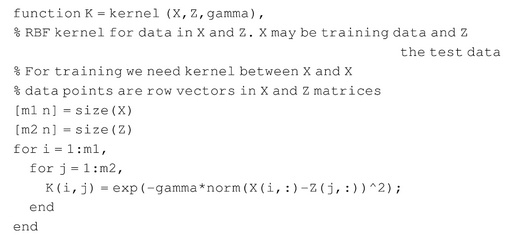
\includegraphics[width=12cm, keepaspectratio,]{fig024.jpg}
	\caption{}
	\label{fig024}
\end{figure} 

Note that actual implementations of this make use of more computationally efficient method \parencite{TFCookbook}. The restated method has a hyper-parameter $\gamma$ that takes the place of $2\sigma^2$. Nevertheless the Scikit-Learn implementation of the RBF kernel has a fit time complexity of more than quadratic to the number of rows of data, making it hard to scale to datasets with more than 10,000 rows. \parencite{chang2011libsvm}.

\subsubsection{RBF Hyper-Parameters}
The RBF-SVM model requires two parameters to be defined, $\gamma$ and C. As explained by \parencite{albon},
gamma is a parameter of the RBF kernel itself and can be thought of as the 'spread' of the kernel and therefore the decision region. When $\gamma$ is low, the 'curve' of the decision boundary is very low and thus the decision region is very broad. When $\gamma$ is high, the 'curve' of the decision boundary is high, which creates islands of decision-boundaries around data points. 
C is a parameter of the SVM optimization and is the penalty for misclassifying a data point. When C is small, the classifier is okay with misclassified data points (high bias, low variance). When C is large, the classifier is heavily penalized for misclassified data and therefore bends over backwards avoid any misclassified data points (low bias, high variance).

\subsection{RNN-LSTM model}

The construction of the RNN model requires a number of hyper-parameters. These are as follows:

\begin{list}{-}
\item Time-steps: How many time steps to use (= batch depth)
\item - Learning rate: Learning rate of backprop algorithm
\item Hidden units: Number of units per hidden layer
	\item Layers: Number of hidden layers
	\item SampleWeighting: Weighting to apply in the cost function for labels that are a play event
	\item User iteration: How many random users to select for training)
	\item SamplesPerUser: How many mini-batches to select for each user
	\item BatchRows: How many random periods to select in each mini-batch (=batch height)
	\item Batch iterations: How many iterations to perform on one batch
\end{list}

\subsubsection{Batch shape}

We provide the RNN model with a sequence of historical data at times $t-1 .. t-n$ with $n >1)$. This is fed into the RNN as separate time steps in forward temporal order (earliest time-steps are processed first). The hidden state would propagate information forward at each time step, until it was used to predict the outcome at time $t$.

Practically speaking this meant feeding in the data with input shape (batch rows, time-steps, features). Some points of interest are:

\begin{enumerate}
	\item The features dimension here only contains $t-1$ and no other feature. 
		
	\item The time-steps are 'unrolled' within Tensorflow and fed into the LSTM. In this research we experiment with different lengths of time-steps, with 48 (half-hour periods ) representing a day, 336 for a week, and 672 for 2 weeks.

	\item When the data is unrolled, time step $t$ for all rows in the batches are processed together as one block, before moving onto the next time-step.

	\item Constructing the 3-d shape often requires building them up in slices. A significant speed up was observed in Python when using a pre-allocated array vs. appending to it.
\end{enumerate}

\subsubsection{Samples and iterations}

A challenge in testing the RNN model was to balance the number of users being samples from, with the number of samples to take from each user, and the number iterations to then do on each sample. A distinction between batch rows and samples per user was required for computational reasons to reduce the demand on RAM per mini-batch, vs. feeding in one large mini-batch per user.

\subsubsection{Cost function and weighting}

Both the logistic loss and a weighted softmax cross entropy loss function were tried in the model (the latter requires converting the output label into one-hot encoding format). Logistic loss was found to be the more effective of the two cost function and hence used for our results. 

Secondly due to the imbalanced data, adding weighting to the costs of a Play event was found to be crucial in getting good results. The key snippet of code for the cost function is given below:

\begin{lstlisting}
_logits = RNN(x, weights, biases,n_steps)
_prob = tf.sigmoid(_logits)
_weightstf.add(1,tf.multiply( _
tf.cast(tf.equal(y,1),'int32'),n_weighting))

_logloss =
tf.losses.log_loss(predictions=_prob, _ labels=y,epsilon=0.00001, _ 
weights=_weights)

_cost = tf.reduce_mean(_logloss)
\end{lstlisting}


\section{Evaluation criteria}

Deciding on an appropriate evaluation measure requires careful consideration to the costs attached to different predictions. In our case the cost of suggesting music when the user is likely not interested is higher than not playing music when they are likely to be interested. 

A number of possible evaluation criteria were looked at. The most-straight forward of which was \textit{accuracy}. This computes the count of correct predictions as a fraction of the total number of predictions. While this is an intuitive measure, it would not distinguish between models that had a high accuracy on the play-events vs. a high accuracy on non-play events. 

To do this we look at precision. Precision (P) is defined as the number of true positives over the number of true positives plus the number of false positives. A positive in this case is a play-event so our precision equation becomes:

$$Precision = \frac{Correct Play Predictions}{Total Play Predictions}$$. 

This will be measuring our models on how many of the 'Play' events predicted were correct. However it does not distinguish between models that predict a play event only on 'safe bets', such as when t-1 was also a play event, vs. those that are attempting to guess the start of a play sequence. For this we turn to recall.

Recall is defined as:

$$Recall = \frac{CorrectPlayPredictions}{TotalPlayPrectionsInDataset}$$

For example if we predicted 100 plays correctly but there were in fact 110 plays in the dataset, then recall would be 100/(100 + 10)= 91%.


\section{Summary}

We have described how our data was transformed to make it useful for our experiments. In particular how we had to convert our list of play events into a list of play and non-play events for every period. By doing this we are faced with an imbalance of data as non-play events make up ~91\% of the data and so we employ a weighting strategy to counteract this.

We then described the methods we will be utilizing in our experiments, consisting of a Baseline model which simply assumes $t =t-1$, a Bayesian model which builds up a weekly profile of listening habits for each user, Logistic and SVM models that apply classical machine learning techniques to our time-series problem, and finally a deep learning model in the form of an RNN-LSTM where we seek to utilize its ability to learn temporal patterns through a hidden memory state.

Finally we looked at different ways for measuring the success of our problem, with precision and recall being the preferred choice.

In the next chapter we shall present the results of our experiments together with insights on each model.